\documentclass[10pt]{beamer}

% Tema Limpo e Profissional
\usetheme{Madrid}
\usecolortheme{whale}

% Pacotes Essenciais
\usepackage[utf8]{inputenc}
\usepackage[portuguese]{babel}
\usepackage{graphicx}
\usepackage{booktabs}
\usepackage{amsmath}
\usepackage{amssymb}
\usepackage{listings}
\usepackage{xcolor}

% Configuracoes de Codigo (Python)
\lstset{
    language=Python,
    basicstyle=\ttfamily\scriptsize,
    keywordstyle=\color{blue}\bfseries,
    stringstyle=\color{red!80!black},
    commentstyle=\color{green!60!black},
    breaklines=true,
    showstringspaces=false,
    tabsize=4
}

% Metadados da Apresentacao
\title[IFCE Tauá - Engenharia de Software]{Aula 20: Introdução à UML, Revisão de OO e Casos de Uso}
\subtitle{Fundamentação Teórica e Prática baseada nos Capítulos 1, 2 e 3 (Gilleanes Guedes)}
\author[Prof. Reginaldo Fernandes]{Prof. Reginaldo Pereira Fernandes\texorpdfstring{\\ \small{Técnico em Informática para Internet}}{}}
\institute[IFCE]{Instituto Federal do Ceará -- Campus Tauá}
\date{\today}

\begin{document}

% -----------------------------------------------------------------------------
% SLIDE 1: Capa
% -----------------------------------------------------------------------------
\begin{frame}
    \titlepage
\end{frame}

% -----------------------------------------------------------------------------
% SLIDE 2: Sumario
% -----------------------------------------------------------------------------
\begin{frame}{Sumário da Aula}
    \tableofcontents
\end{frame}

% =============================================================================
\section{Introdução à UML e Importância da Modelagem (Cap. 1)}
% =============================================================================

% -----------------------------------------------------------------------------
% SLIDE 3: O Paradoxo da Construção
% -----------------------------------------------------------------------------
\begin{frame}{Por que Modelar Software? O Paradoxo da Construção}
    \begin{columns}
        \begin{column}{0.55\textwidth}
            \textbf{A Metáfora da Construção Civil:}
            \begin{itemize}
                \item \textbf{Casinha de cachorro:} Qualquer pessoa constrói em poucas horas sem projeto. Se cair, o prejuízo é desprezível.
                \item \textbf{Casa de um andar:} Exige esboços básicos, mas desvios são toleráveis e corrigíveis.
                \item \textbf{Edifício de vários andares:} Jamais se inicia a obra sem plantas arquitetônica, hidráulica, elétrica e estrutural!
            \end{itemize}
            \vspace{0.2cm}
            \textbf{No Software Moderno:}
            \begin{itemize}
                \item Sistemas corporativos e aplicações web comerciais operam como edifícios: envolvem regras de negócio, dados, segurança e alta concorrência.
            \end{itemize}
        \end{column}
        \begin{column}{0.45\textwidth}
            \begin{block}{Custo do Retrabalho}
                Corrigir uma falha estrutural de requisitos na fase de codificação ou em produção pode custar até \textbf{100 vezes mais} do que identificá-la na modelagem.
            \end{block}
            \vspace{0.2cm}
            \begin{exampleblock}{Fatores de Mudança Contínua}
                \begin{itemize}
                    \item Mudanças no mercado;
                    \item Novas exigências tributárias e legais;
                    \item Evolução contínua das demandas do cliente.
                \end{itemize}
            \end{exampleblock}
        \end{column}
    \end{columns}
\end{frame}

% -----------------------------------------------------------------------------
% SLIDE 4: Elicitação, Requisitos e Prototipação
% -----------------------------------------------------------------------------
\begin{frame}{Elicitação de Requisitos e Prototipação}
    \begin{columns}
        \begin{column}{0.52\textwidth}
            \textbf{O Domínio do Problema:}
            \begin{itemize}
                \item \textbf{Requisitos Funcionais (RF):} O que o sistema deve fazer (ex.: cadastrar cliente, emitir extrato, processar pedido).
                \item \textbf{Requisitos Não Funcionais (RNF):} Como o sistema deve operar (ex.: tempo de resposta, padrões de segurança, escalabilidade, regras de negócio).
            \end{itemize}
            \vspace{0.2cm}
            \textbf{Ruídos de Comunicação:}
            \begin{itemize}
                \item O cliente relata necessidades usando termos vagos de negócio; o desenvolvedor raciocina com bancos de dados e código.
            \end{itemize}
        \end{column}
        \begin{column}{0.48\textwidth}
            \begin{block}{A Técnica da Prototipação (RAD)}
                Desenvolver telas e protótipos de baixa ou alta fidelidade valida requisitos com o usuário antes de codificar.
            \end{block}
            \vspace{0.2cm}
            \begin{alertblock}{O que é um Modelo de Software?}
                É uma abstração simplificada que omite detalhes secundários para focar nos aspectos essenciais sob uma perspectiva específica.
            \end{alertblock}
        \end{column}
    \end{columns}
\end{frame}

% -----------------------------------------------------------------------------
% SLIDE 5: Historico da UML
% -----------------------------------------------------------------------------
\begin{frame}{Breve Histórico da UML: Da Fragmentação ao Padrão}
    \begin{columns}
        \begin{column}{0.55\textwidth}
            \textbf{A ``Guerra dos Métodos'' (Início dos Anos 90):}
            \begin{itemize}
                \item Dezenas de metodologias concorrentes disputavam o mercado, gerando incompatibilidade de notações entre equipes.
            \end{itemize}
            \vspace{0.2cm}
            \textbf{Os ``Três Amigos'' (Three Amigos):}
            \begin{itemize}
                \item \textbf{Grady Booch:} Criador do Método Booch;
                \item \textbf{James Rumbaugh:} Criador do Método OMT (\textit{Object Modeling Technique});
                \item \textbf{Ivar Jacobson:} Criador do Método OOSE (\textit{Object-Oriented Software Engineering} - pioneiro dos Casos de Uso).
            \end{itemize}
        \end{column}
        \begin{column}{0.45\textwidth}
            \begin{block}{A Padronização pela OMG}
                \begin{itemize}
                    \item Reunidos na \textbf{Rational Software}, unificaram seus métodos no \textbf{Método Unificado} (1995);
                    \item Em 1997, a \textbf{OMG} (\textit{Object Management Group}) adotou a UML 1.1 como padrão global;
                    \item Em 2005, lançamento da \textbf{UML 2.0}, trazendo forte reestruturação em 14 diagramas oficiais.
                \end{itemize}
            \end{block}
        \end{column}
    \end{columns}
\end{frame}

% -----------------------------------------------------------------------------
% SLIDE 6: Por que Tantos Diagramas?
% -----------------------------------------------------------------------------
\begin{frame}{Por que a UML Possui Tantos Diagramas?}
    \begin{itemize}
        \item \textbf{Múltiplas Visões Complementares:} Um software complexo não pode ser compreendido satisfatoriamente sob uma única perspectiva sem sobrecarregar a notação.
        \item \textbf{Públicos e Níveis de Abstração Distintos:}
        \begin{itemize}
            \item \textbf{Clientes e Analistas de Negócio:} Necessitam de diagramas conceituais de alto nível (ex.: Casos de Uso, Atividades);
            \item \textbf{Arquitetos e Desenvolvedores:} Necessitam de diagramas técnicos de projeto (ex.: Classes, Sequência, Componentes);
            \item \textbf{Engenheiros de Infraestrutura/DevOps:} Necessitam de diagramas físicos de hardware e rede (ex.: Implantação).
        \end{itemize}
    \end{itemize}
    \vspace{0.3cm}
    \begin{block}{Analogia com a Engenharia Civil}
        Assim como um edifício requer plantas distintas (arquitetônica, hidráulica, sanitária e elétrica), a UML fornece 14 diagramas especializados para cada dimensão do sistema.
    \end{block}
\end{frame}

% -----------------------------------------------------------------------------
% SLIDE 7: Taxonomia Geral da UML 2 (Slide de Pagina Unica)
% -----------------------------------------------------------------------------
\begin{frame}{Taxonomia Oficial dos 14 Diagramas da UML 2}
    \centering
    \textbf{Organograma Geral da UML 2 (Figura 1.15 do Livro):}\\[0.2cm]
    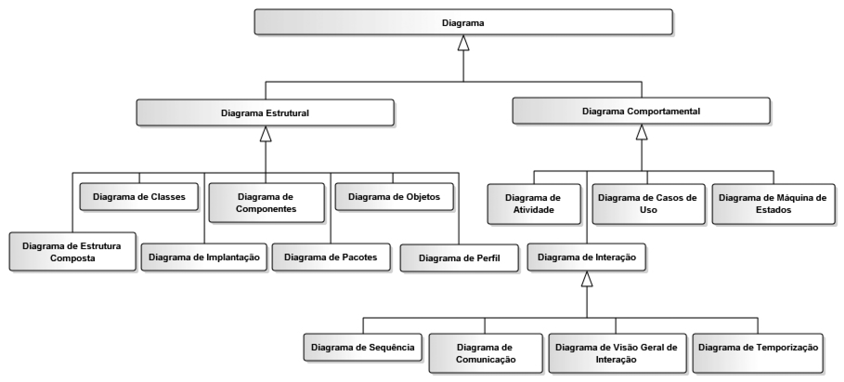
\includegraphics[width=0.92\textwidth,height=0.65\textheight,keepaspectratio]{imagens/Fig1.15.png}\\[0.2cm]
    \scriptsize A UML divide-se em 7 Diagramas Estruturais e 7 Diagramas Comportamentais (incluindo 4 de Interação).
\end{frame}

% -----------------------------------------------------------------------------
% SLIDE 8: Galeria Estrutural: Diagrama de Classes (Pagina Unica)
% -----------------------------------------------------------------------------
\begin{frame}{Diagrama de Classes: Visão Geral}
    \centering
    \textbf{Exemplo de Diagrama de Classes (Figura 1.2 do Livro):}\\[0.2cm]
    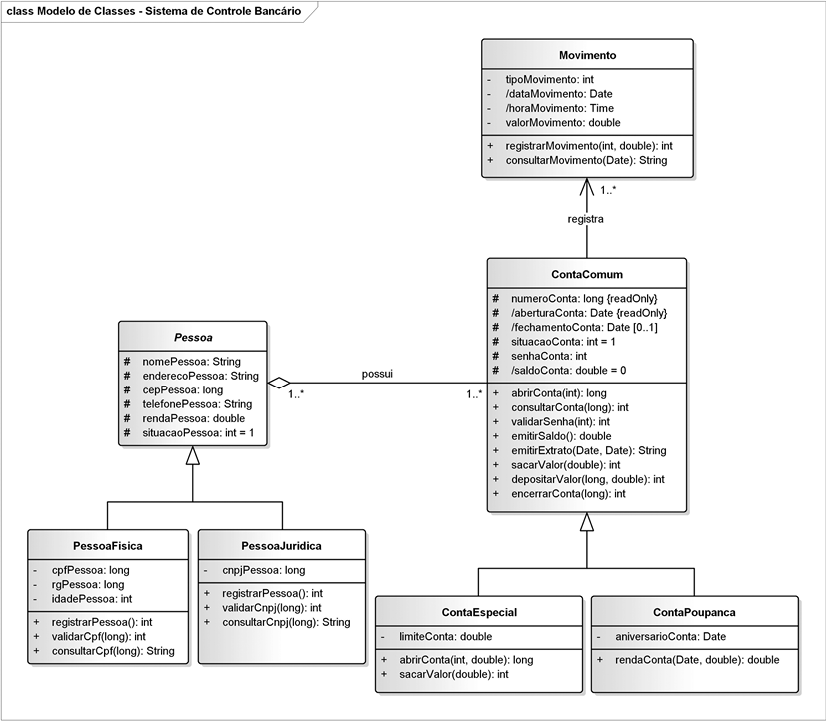
\includegraphics[width=0.9\textwidth,height=0.72\textheight,keepaspectratio]{imagens/Fig1.2.png}\\[0.15cm]
    \scriptsize É o diagrama estrutural mais importante da UML, exibindo classes, atributos, métodos e associações estáticas.
\end{frame}

% -----------------------------------------------------------------------------
% SLIDE 9: Galeria Estrutural: Diagrama de Pacotes (Pagina Unica)
% -----------------------------------------------------------------------------
\begin{frame}{Diagrama de Pacotes: Organização em Módulos}
    \centering
    \textbf{Exemplo de Diagrama de Pacotes (Figura 1.4 do Livro):}\\[0.2cm]
    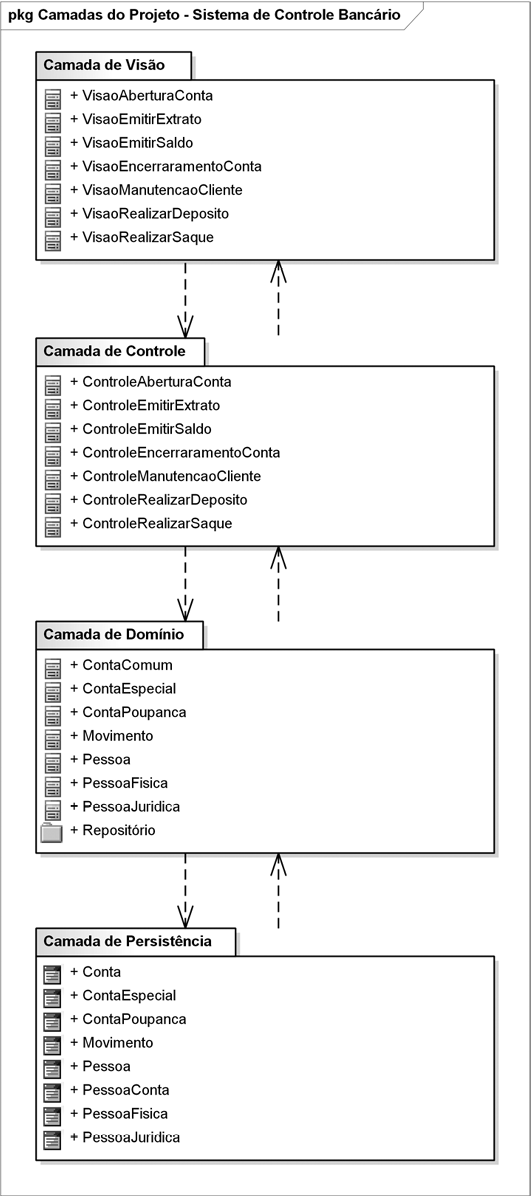
\includegraphics[width=0.9\textwidth,height=0.72\textheight,keepaspectratio]{imagens/Fig1.4.png}\\[0.15cm]
    \scriptsize Agrupa elementos do modelo logicamente em subsistemas ou camadas arquiteturais (Apresentação, Negócio, Acesso a Dados).
\end{frame}

% -----------------------------------------------------------------------------
% SLIDE 10: Galeria Comportamental: Diagrama de Sequência (Pagina Unica)
% -----------------------------------------------------------------------------
\begin{frame}{Diagrama de Sequência: Interação Temporal}
    \centering
    \textbf{Exemplo de Diagrama de Sequência (Figura 1.5 do Livro):}\\[0.2cm]
    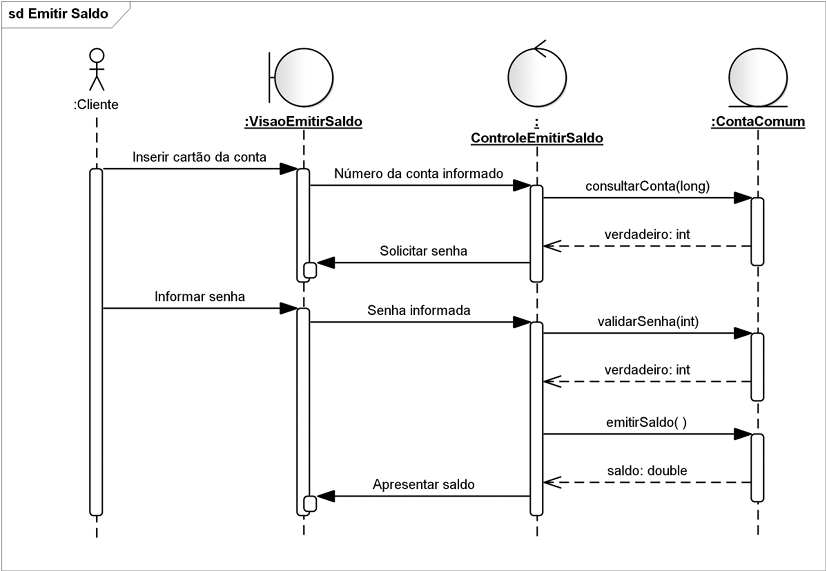
\includegraphics[width=0.92\textwidth,height=0.70\textheight,keepaspectratio]{imagens/Fig1.5.png}\\[0.15cm]
    \scriptsize Enfatiza a ordem cronológica em que mensagens e dados são trocados entre objetos ao longo de suas linhas de vida.
\end{frame}

% -----------------------------------------------------------------------------
% SLIDE 11: Galeria Comportamental: Máquina de Estados e Atividades
% -----------------------------------------------------------------------------
\begin{frame}{Máquina de Estados e Atividades (Página Única)}
    \begin{columns}
        \begin{column}{0.5\textwidth}
            \centering
            \textbf{Máquina de Estados (Fig. 1.7):}\\[0.15cm]
            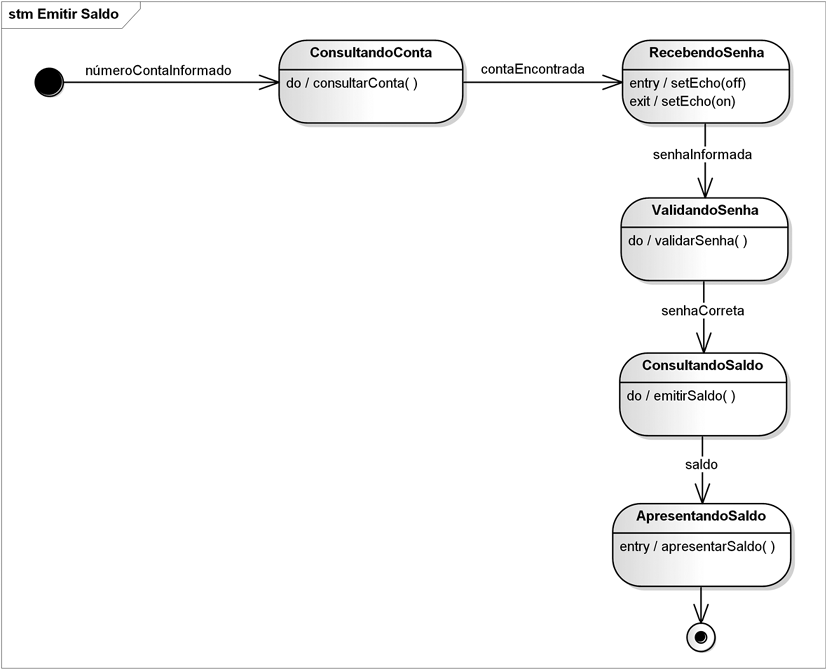
\includegraphics[width=\columnwidth,height=0.62\textheight,keepaspectratio]{imagens/Fig1.7.png}\\[0.1cm]
            \scriptsize Ciclo de vida e transições de estado de um objeto sob eventos.
        \end{column}
        \begin{column}{0.5\textwidth}
            \centering
            \textbf{Atividade (Fig. 1.8):}\\[0.15cm]
            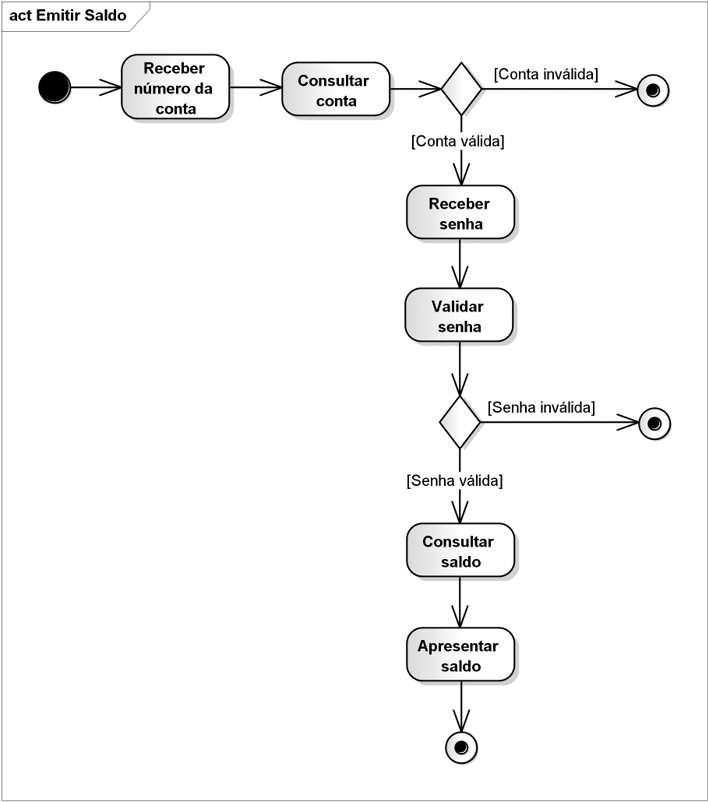
\includegraphics[width=\columnwidth,height=0.62\textheight,keepaspectratio]{imagens/Fig1.8.png}\\[0.1cm]
            \scriptsize Fluxo sequencial e paralelo de passos, decisões e algoritmos.
        \end{column}
    \end{columns}
\end{frame}

% -----------------------------------------------------------------------------
% SLIDE 12: Galeria Estrutural: Diagrama de Implantação (Pagina Unica)
% -----------------------------------------------------------------------------
\begin{frame}{Diagrama de Implantação: Arquitetura Física}
    \centering
    \textbf{Exemplo de Diagrama de Implantação (Figura 1.11 do Livro):}\\[0.2cm]
    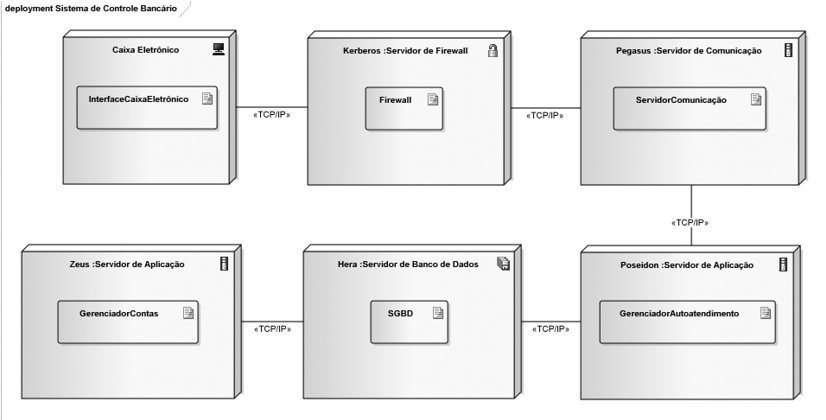
\includegraphics[width=0.92\textwidth,height=0.70\textheight,keepaspectratio]{imagens/Fig1.11.png}\\[0.15cm]
    \scriptsize Especifica o hardware, servidores de aplicação, bancos de dados, estações cliente e protocolos de comunicação física.
\end{frame}

% =============================================================================
\section{Revisão de Orientação a Objetos (Cap. 2)}
% =============================================================================

% -----------------------------------------------------------------------------
% SLIDE 13: Conceitos Fundamentais de OO
% -----------------------------------------------------------------------------
\begin{frame}{O Paradigma de Orientação a Objetos}
    \begin{columns}
        \begin{column}{0.55\textwidth}
            \textbf{Fundamentação Cognitiva:}
            \begin{itemize}
                \item O pensamento humano categoriza e abstrai a realidade continuamente através de moldes conceituais (ex.: o conceito geral de ``carro'' ou ``pessoa'').
            \end{itemize}
            \vspace{0.2cm}
            \textbf{Pilares Essenciais:}
            \begin{itemize}
                \item \textbf{Abstração:} Isolar as características essenciais para o contexto do sistema, descartando detalhes irrelevantes.
                \item \textbf{Classificação:} Definir o modelo (molde) que agrupa características e comportamentos comuns.
                \item \textbf{Instanciação:} Materializar um objeto individual na memória com valores concretos em seus atributos.
            \end{itemize}
        \end{column}
        \begin{column}{0.45\textwidth}
            \begin{block}{Classe vs. Objeto}
                \begin{itemize}
                    \item \textbf{Classe:} Planta baixa, tipo de dado abstrato, definição estrutural.
                    \item \textbf{Objeto:} Instância real em memória, com identidade, estado e comportamento.
                \end{itemize}
            \end{block}
            \vspace{0.2cm}
            \begin{alertblock}{Estado de um Objeto}
                O conjunto de valores armazenados em seus atributos em um dado instante define o seu estado.
            \end{alertblock}
        \end{column}
    \end{columns}
\end{frame}

% -----------------------------------------------------------------------------
% SLIDE 14: Anatomia de uma Classe na UML: Evolução dos Compartimentos
% -----------------------------------------------------------------------------
\begin{frame}{Anatomia de uma Classe na UML: 3 Divisões}
    Na UML, uma classe é representada por um retângulo com até \textbf{três divisões}:
    \vspace{0.25cm}
    \begin{columns}
        \begin{column}{0.33\textwidth}
            \centering
            \textbf{1. Apenas Nome (2.1)}\\[0.2cm]
            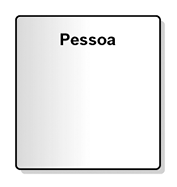
\includegraphics[height=0.35\textheight]{imagens/Fig2.1.png}\\[0.2cm]
            \scriptsize Visão condensada: nome centralizado e destacado.
        \end{column}
        \begin{column}{0.33\textwidth}
            \centering
            \textbf{2. Com Atributos (2.2)}\\[0.2cm]
            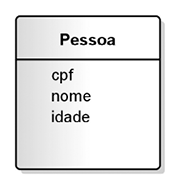
\includegraphics[height=0.35\textheight]{imagens/Fig2.2.png}\\[0.2cm]
            \scriptsize 2ª divisão: propriedades que compõem o estado.
        \end{column}
        \begin{column}{0.33\textwidth}
            \centering
            \textbf{3. Com Métodos (2.3)}\\[0.2cm]
            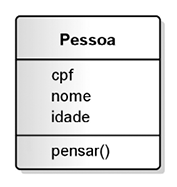
\includegraphics[height=0.35\textheight]{imagens/Fig2.3.png}\\[0.2cm]
            \scriptsize 3ª divisão: operações e comportamentos executáveis.
        \end{column}
    \end{columns}
\end{frame}

% -----------------------------------------------------------------------------
% SLIDE 15: Visibilidade e Tipos (Pagina Unica)
% -----------------------------------------------------------------------------
\begin{frame}{Modificadores de Visibilidade e Tipos}
    \begin{columns}
        \begin{column}{0.55\textwidth}
            \textbf{Notação de Visibilidade na UML:}
            \begin{itemize}
                \item \textbf{Pública (\texttt{+}):} Acessível por qualquer classe externa;
                \item \textbf{Privada (\texttt{-}):} Acessível exclusivamente por métodos da própria classe;
                \item \textbf{Protegida (\texttt{\#}):} Acessível pela própria classe e por suas subclasses derivadas;
                \item \textbf{Pacote (\texttt{\~{}}):} Acessível por elementos pertencentes ao mesmo pacote.
            \end{itemize}
            \vspace{0.2cm}
            \begin{block}{Encapsulamento}
                Atributos costumam ser \textbf{privados} ou \textbf{protegidos}, enquanto operações públicas formam a interface de comunicação segura.
            \end{block}
        \end{column}
        \begin{column}{0.45\textwidth}
            \centering
            \textbf{Classe Completa (Figura 2.4):}\\[0.15cm]
            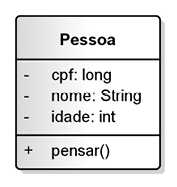
\includegraphics[width=\columnwidth,height=0.62\textheight,keepaspectratio]{imagens/Fig2.4.png}
        \end{column}
    \end{columns}
\end{frame}

% -----------------------------------------------------------------------------
% SLIDE 16: Herança: Hierarquia Animal (Pagina Unica)
% -----------------------------------------------------------------------------
\begin{frame}{Herança: Generalização e Especialização}
    \begin{columns}
        \begin{column}{0.5\textwidth}
            \textbf{Mecanismo de Reuso:}
            \begin{itemize}
                \item \textbf{Superclasse (Mãe/Base):} Define atributos e métodos genéricos compartilhados.
                \item \textbf{Subclasse (Filha/Derivada):} Herda os membros da superclasse e acrescenta características exclusivas.
            \end{itemize}
            \vspace{0.2cm}
            \textbf{Vantagens:}
            \begin{itemize}
                \item Reutilização direta de código testado;
                \item Facilidade de manutenção centralizada;
                \item Extensibilidade sem duplicação de lógica.
            \end{itemize}
        \end{column}
        \begin{column}{0.5\textwidth}
            \centering
            \textbf{Hierarquia Animal (Figura 2.5):}\\[0.15cm]
            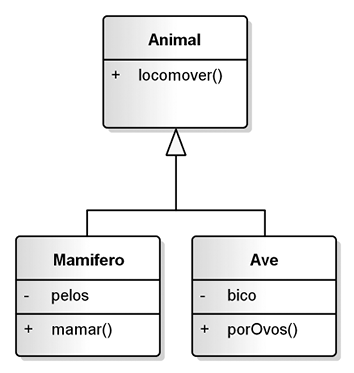
\includegraphics[width=\columnwidth,height=0.65\textheight,keepaspectratio]{imagens/Fig2.5.png}
        \end{column}
    \end{columns}
\end{frame}

% -----------------------------------------------------------------------------
% SLIDE 17: Herança Múltipla: Caso do Ornitorrinco (Pagina Unica)
% -----------------------------------------------------------------------------
\begin{frame}{Herança Múltipla na Prática}
    \begin{columns}
        \begin{column}{0.5\textwidth}
            \textbf{Conceito:}
            \begin{itemize}
                \item Uma subclasse herda diretamente atributos e métodos de \textbf{duas ou mais} superclasses simultaneamente.
            \end{itemize}
            \vspace{0.2cm}
            \textbf{O Exemplo de Guedes (Figura 2.6):}
            \begin{itemize}
                \item O \texttt{Ornitorrinco} herda pelos e capacidade de mamar da classe \texttt{Mamifero};
                \item Herda bico e capacidade de pôr ovos da classe \texttt{Ave};
                \item Herda a capacidade de locomoção da superclasse comum \texttt{Animal}.
            \end{itemize}
        \end{column}
        \begin{column}{0.5\textwidth}
            \centering
            \textbf{Herança Múltipla (Figura 2.6):}\\[0.15cm]
            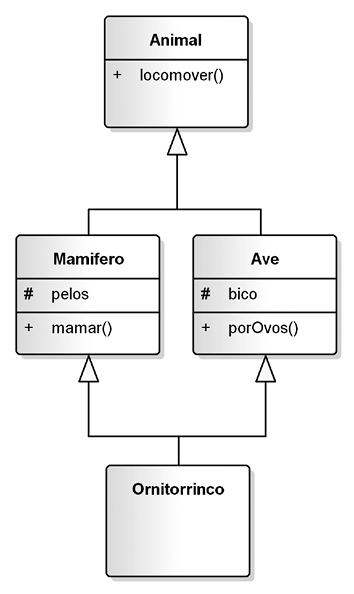
\includegraphics[width=\columnwidth,height=0.72\textheight,keepaspectratio]{imagens/Fig2.6.png}
        \end{column}
    \end{columns}
\end{frame}

% -----------------------------------------------------------------------------
% SLIDE 18: Polimorfismo e Sobrescrita (Pagina Unica)
% -----------------------------------------------------------------------------
\begin{frame}{Polimorfismo e Sobrescrita de Métodos}
    \begin{columns}
        \begin{column}{0.5\textwidth}
            \textbf{Conceito Central:}
            \begin{itemize}
                \item ``Muitas formas'': capacidade de objetos de subclasses distintas responderem à \textbf{mesma mensagem} com comportamentos especializados.
            \end{itemize}
            \vspace{0.2cm}
            \textbf{O Caso Bancário (Figura 2.7):}
            \begin{itemize}
                \item \texttt{ContaComum}: possui \texttt{\#saldo} e método \texttt{+saque()}, restrito ao saldo existente;
                \item \texttt{ContaEspecial}: adiciona \texttt{\#limite} e sobrescreve (\textit{override}) o método \texttt{+saque()} para permitir saque até a soma de saldo e limite.
            \end{itemize}
        \end{column}
        \begin{column}{0.5\textwidth}
            \centering
            \textbf{Modelo Polimórfico (Figura 2.7):}\\[0.15cm]
            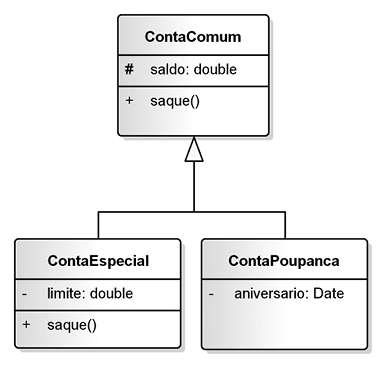
\includegraphics[width=\columnwidth,height=0.68\textheight,keepaspectratio]{imagens/Fig2.7.png}
        \end{column}
    \end{columns}
\end{frame}

% -----------------------------------------------------------------------------
% SLIDE 19: Codigo Python ContaComum e ContaEspecial
% -----------------------------------------------------------------------------
\begin{frame}[fragile]{Mapeamento Conceitual: Do Modelo ao Código}
    No arquivo \texttt{exemplo\_poo.py}, o modelo da Figura 2.7 é implementado:
\begin{lstlisting}
class ContaComum:
    def __init__(self, numero: str, saldo: float = 0.0):
        self._saldo = float(saldo)  # Protegido (#)
    def saque(self, valor: float) -> bool:
        if 0 < valor <= self._saldo:
            self._saldo -= valor
            return True
        return False

class ContaEspecial(ContaComum):
    def __init__(self, numero: str, saldo: float = 0.0, limite: float = 500.0):
        super().__init__(numero, saldo)
        self._limite = float(limite)  # Protegido (#)
    def saque(self, valor: float) -> bool:  # Sobrescrita Polimorfica
        if 0 < valor <= (self._saldo + self._limite):
            self._saldo -= valor      # Saldo pode ficar negativo
            return True
        return False
\end{lstlisting}
\end{frame}

% =============================================================================
\section{Diagrama de Casos de Uso (Cap. 3)}
% =============================================================================

% -----------------------------------------------------------------------------
% SLIDE 20: O que é o Diagrama de Casos de Uso?
% -----------------------------------------------------------------------------
\begin{frame}{O que é o Diagrama de Casos de Uso?}
    \begin{columns}
        \begin{column}{0.55\textwidth}
            \textbf{Finalidade Central:}
            \begin{itemize}
                \item Criado originalmente por \textbf{Ivar Jacobson} em 1986 (metodologia OOSE).
                \item Apresenta uma visão externa de \textbf{``caixa-preta''} do sistema.
                \item Mapeia \textbf{quem} interage com o sistema e \textbf{quais serviços de valor} o sistema disponibiliza.
            \end{itemize}
            \vspace{0.2cm}
            \begin{block}{O que NÃO é Casos de Uso?}
                Não se preocupa com telas, bancos de dados, linguagens ou algoritmos internos. O foco reside nas funcionalidades do usuário!
            \end{block}
        \end{column}
        \begin{column}{0.45\textwidth}
            \begin{alertblock}{Elemento de Ligação}
                O diagrama de casos de uso é a principal ponte de comunicação entre clientes e a equipe de desenvolvimento.
            \end{alertblock}
            \vspace{0.2cm}
            \textbf{Elementos Centrais:}
            \begin{enumerate}
                \item Atores;
                \item Casos de Uso;
                \item Associações;
                \item Fronteira de Sistema.
            \end{enumerate}
        \end{column}
    \end{columns}
\end{frame}

% -----------------------------------------------------------------------------
% SLIDE 21: Atores (Figura 3.1)
% -----------------------------------------------------------------------------
\begin{frame}{Atores no Diagrama de Casos de Uso}
    \begin{columns}
        \begin{column}{0.55\textwidth}
            \textbf{Definição de Ator:}
            \begin{itemize}
                \item Representa um \textbf{papel} desempenhado por uma entidade externa que interage diretamente com o sistema.
                \item \textbf{Atores Humanos:} Clientes, Gerentes, Atendentes, Entregadores.
                \item \textbf{Atores Não Humanos (Sistemas Externos):} Gateways de pagamento, servidores de e-mail, APIs de frete, sensores.
            \end{itemize}
            \vspace{0.2cm}
            \textbf{Como Identificar os Atores?}
            \begin{itemize}
                \item Quem fornecerá dados ao sistema?
                \item Quem consumirá as saídas e relatórios?
                \item Quais sistemas externos realizam trocas de informações?
            \end{itemize}
        \end{column}
        \begin{column}{0.45\textwidth}
            \centering
            \textbf{Representação do Ator (3.1):}\\[0.2cm]
            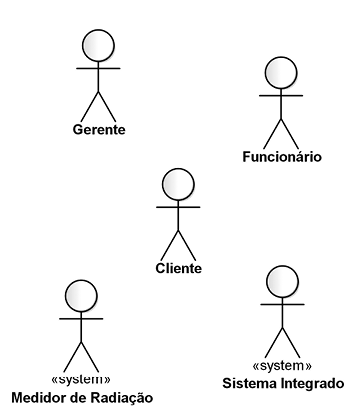
\includegraphics[height=0.45\textheight]{imagens/Fig3.1.png}\\[0.2cm]
            \scriptsize Boneco palito (\textit{stickman}) com nome do papel abaixo.
        \end{column}
    \end{columns}
\end{frame}

% -----------------------------------------------------------------------------
% SLIDE 22: Casos de Uso e Associações (Figuras 3.2 e 3.3)
% -----------------------------------------------------------------------------
\begin{frame}{Casos de Uso e Associações}
    \begin{columns}
        \begin{column}{0.5\textwidth}
            \textbf{O que é um Caso de Uso? (3.2)}
            \begin{itemize}
                \item Representa uma funcionalidade ou serviço completo entregue pelo sistema.
                \item Graficamente é uma \textbf{elipse}.
                \item \textbf{Regra de Nomeação:} Verbo no infinitivo seguido de substantivo (ex.: \textit{Consultar Saldo}, \textit{Finalizar Pedido}).
            \end{itemize}
            \centering
            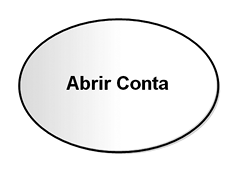
\includegraphics[width=0.85\columnwidth]{imagens/Fig3.2.png}
        \end{column}
        \begin{column}{0.5\textwidth}
            \textbf{Associação com Ator (3.3)}
            \begin{itemize}
                \item Uma linha contínua conectando o ator ao caso de uso.
                \item Indica comunicação direta: o ator inicia o caso de uso ou recebe dados dele.
            \end{itemize}
            \centering
            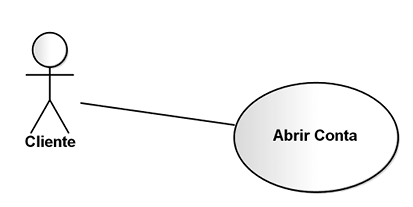
\includegraphics[width=0.85\columnwidth]{imagens/Fig3.3.png}
        \end{column}
    \end{columns}
\end{frame}

% -----------------------------------------------------------------------------
% SLIDE 23: Generalização/Especialização (Figuras 3.4 e 3.5)
% -----------------------------------------------------------------------------
\begin{frame}{Generalização e Especialização}
    \begin{columns}
        \begin{column}{0.5\textwidth}
            \textbf{Entre Casos de Uso (3.4):}
            \begin{itemize}
                \item O caso filho herda o comportamento do caso pai e especializa etapas específicas.
                \item Exemplo: \textit{Abrir Conta Especial} herda de \textit{Abrir Conta}.
            \end{itemize}
            \centering
            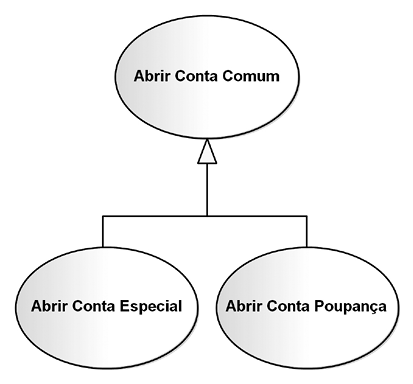
\includegraphics[height=0.35\textheight]{imagens/Fig3.4.png}
        \end{column}
        \begin{column}{0.5\textwidth}
            \textbf{Entre Atores (3.5):}
            \begin{itemize}
                \item Um ator especializado herda todos os casos de uso do ator mais geral.
                \item Exemplo: \textit{Cliente Especial} herda todos os direitos de \textit{Cliente Comum}.
            \end{itemize}
            \centering
            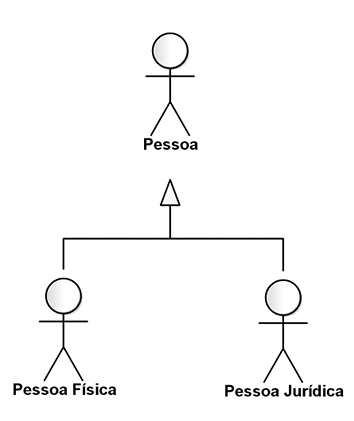
\includegraphics[height=0.35\textheight]{imagens/Fig3.5.png}
        \end{column}
    \end{columns}
\end{frame}

% -----------------------------------------------------------------------------
% SLIDE 24: Relacionamento de Inclusão <<include>> (Pagina Unica)
% -----------------------------------------------------------------------------
\begin{frame}{Relacionamento de Inclusão (\texttt{<<include>>})}
    \begin{columns}
        \begin{column}{0.55\textwidth}
            \textbf{Conceito Central:}
            \begin{itemize}
                \item Utilizado quando uma sequência de passos é \textbf{comum a múltiplos casos de uso}.
                \item A execução do caso de uso incluído é \textbf{OBRIGATÓRIA}!
                \item O caso base não se completa sem o término com sucesso do caso incluído.
                \item Evita redundância de especificação.
            \end{itemize}
            \vspace{0.15cm}
            \begin{alertblock}{Direção da Seta no Include}
                A seta aponta do \textbf{Caso Base} para o \textbf{Caso Incluído}:
                \vspace{0.05cm}
                \centering
                \scriptsize \texttt{Caso Base} $\;\xrightarrow{\;\text{include}\;}\;$ \texttt{Caso Incluído}
            \end{alertblock}
        \end{column}
        \begin{column}{0.45\textwidth}
            \centering
            \textbf{Exemplo do Livro (3.7):}\\[0.1cm]
            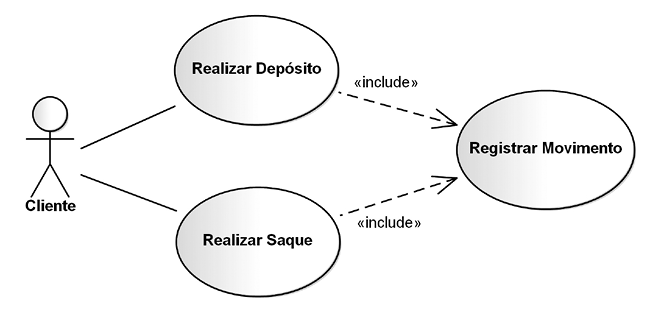
\includegraphics[width=\columnwidth,height=0.45\textheight,keepaspectratio]{imagens/Fig3.7.png}\\[0.1cm]
            \scriptsize Saque e Depósito incluem obrigatoriamente Registrar Movimento.
        \end{column}
    \end{columns}
\end{frame}

% -----------------------------------------------------------------------------
% SLIDE 25: Relacionamento de Extensão <<extend>> (Pagina Unica)
% -----------------------------------------------------------------------------
\begin{frame}{Relacionamento de Extensão (\texttt{<<extend>>})}
    \begin{columns}
        \begin{column}{0.55\textwidth}
            \textbf{Conceito Central:}
            \begin{itemize}
                \item Utilizado para modelar fluxos e cenários \textbf{OPCIONAIS} ou \textbf{CONDICIONAIS}.
                \item O caso de uso extensor só é acionado sob certas circunstâncias ou decisão do usuário.
                \item O caso base pode ser concluído normalmente sem a execução do caso estendido.
            \end{itemize}
            \vspace{0.15cm}
            \begin{alertblock}{Direção da Seta no Extend}
                A seta aponta do \textbf{Caso Extensor} (opcional) para o \textbf{Caso Base}:
                \vspace{0.05cm}
                \centering
                \scriptsize \texttt{Caso Extensor} $\;\xrightarrow{\;\text{extend}\;}\;$ \texttt{Caso Base}
            \end{alertblock}
        \end{column}
        \begin{column}{0.45\textwidth}
            \centering
            \textbf{Exemplo com Restrição (3.12):}\\[0.1cm]
            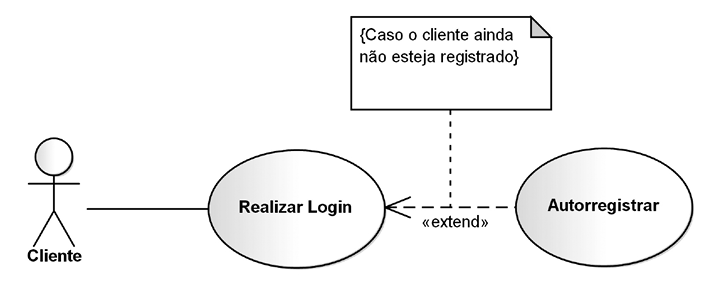
\includegraphics[width=\columnwidth,height=0.45\textheight,keepaspectratio]{imagens/Fig3.12.png}\\[0.1cm]
            \scriptsize Autorregistrar estende Realizar Login caso o cliente não tenha cadastro.
        \end{column}
    \end{columns}
\end{frame}

% -----------------------------------------------------------------------------
% SLIDE 26: Pontos de Extensão (Pagina Unica)
% -----------------------------------------------------------------------------
\begin{frame}{Pontos de Extensão (\textit{Extension Points})}
    \begin{columns}
        \begin{column}{0.52\textwidth}
            \textbf{O que é um Ponto de Extensão?}
            \begin{itemize}
                \item Identifica exatamente \textbf{em qual etapa} do caso de uso base o comportamento opcional pode ser disparado.
                \item Na elipse da UML, cria-se um compartimento inferior nomeado com os pontos de extensão.
            \end{itemize}
            \vspace{0.15cm}
            \begin{exampleblock}{Caso do Livro de Guedes (3.14)}
                Ao \textit{Encerrar Conta}, os pontos de extensão verificam:
                \begin{itemize}
                    \item Se saldo positivo: dispara \textit{Realizar Saque};
                    \item Se saldo negativo: dispara \textit{Cobrar Débito}.
                \end{itemize}
            \end{exampleblock}
        \end{column}
        \begin{column}{0.48\textwidth}
            \centering
            \textbf{Pontos de Extensão (Figura 3.14):}\\[0.1cm]
            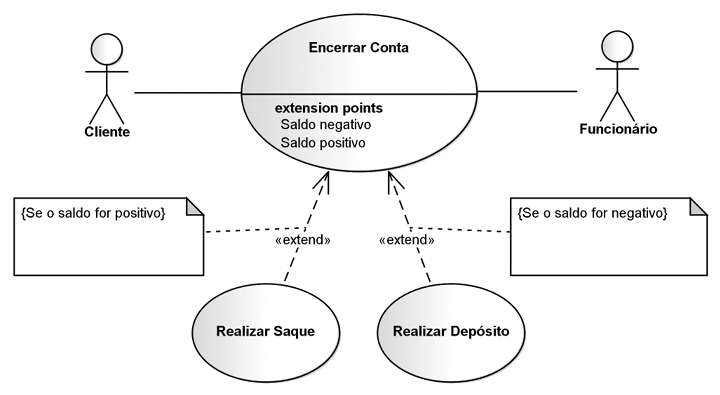
\includegraphics[width=\columnwidth,height=0.55\textheight,keepaspectratio]{imagens/Fig3.14.png}
        \end{column}
    \end{columns}
\end{frame}

% -----------------------------------------------------------------------------
% SLIDE 27: Fronteira do Sistema: Sistema Bancário (Pagina Unica)
% -----------------------------------------------------------------------------
\begin{frame}{Fronteira do Sistema: Sistema Bancário Completo}
    \centering
    \textbf{Fronteira do Sistema e Casos de Uso (Figura 3.17 do Livro):}\\[0.15cm]
    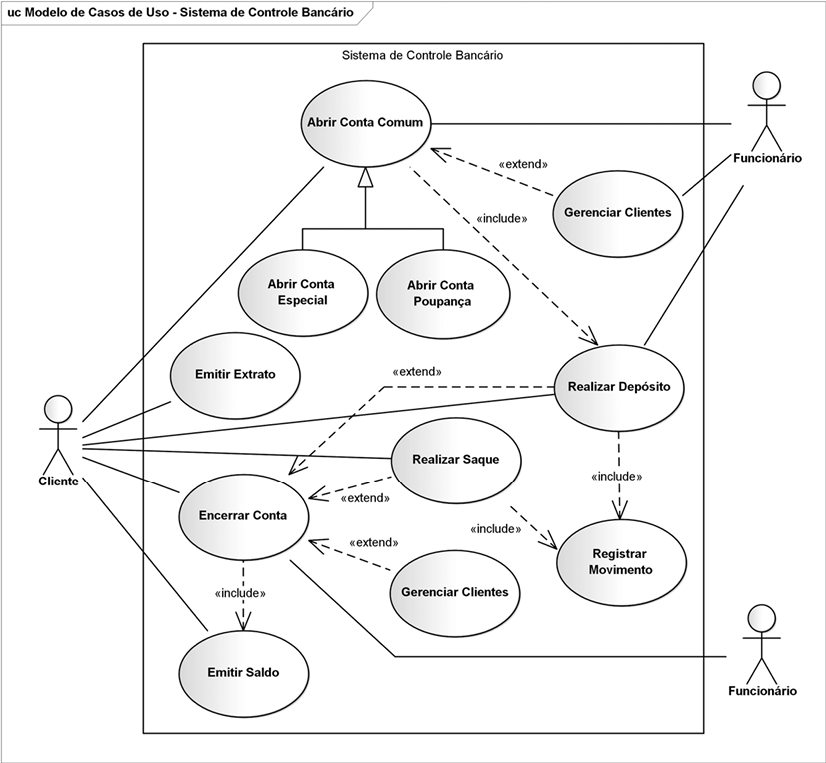
\includegraphics[width=0.92\textwidth,height=0.72\textheight,keepaspectratio]{imagens/Fig3.17.png}\\[0.1cm]
    \scriptsize O retângulo delimita o software: Casos de Uso ficam DENTRO; Atores ficam FORA.
\end{frame}

% -----------------------------------------------------------------------------
% SLIDE 28: Documentação Textual de Casos de Uso
% -----------------------------------------------------------------------------
\begin{frame}{Documentação Textual de Casos de Uso}
    Gilleanes Guedes destaca: \textbf{o diagrama não é suficiente!} Ele precisa ser acompanhado da especificação detalhada de cenários:
    \vspace{0.1cm}
    \begin{block}{Campos Padronizados da Ficha Técnica (Seção 3.4 do Livro)}
        \footnotesize
        \begin{itemize}
            \item \textbf{Identificador e Nome:} Código único e verbo de ação (ex.: \textit{UC03 - Finalizar Pedido}).
            \item \textbf{Atores Envolvidos:} Ator primário (iniciador) e secundários (sistemas de apoio).
            \item \textbf{Pré-condições:} Requisitos que devem ser verdadeiros antes do início do fluxo.
            \item \textbf{Pós-condições:} Estado garantido do sistema após execução com sucesso.
            \item \textbf{Fluxo Principal (Caminho Feliz):} Sequência ordenada de passos onde tudo ocorre com sucesso.
            \item \textbf{Fluxos Alternativos:} Caminhos secundários de navegação ou decisões opcionais do usuário.
            \item \textbf{Fluxos de Exceção:} Tratamento de erros, falhas técnicas e validações frustradas.
        \end{itemize}
    \end{block}
\end{frame}

% -----------------------------------------------------------------------------
% SLIDE 29: Estudo de Caso: Telefonia Celular (Pagina Unica)
% -----------------------------------------------------------------------------
\begin{frame}{Estudo de Caso: Sistema de Telefonia Celular}
    \centering
    \textbf{Diagrama de Casos de Uso - Telefonia (Figura 3.18 do Livro):}\\[0.15cm]
    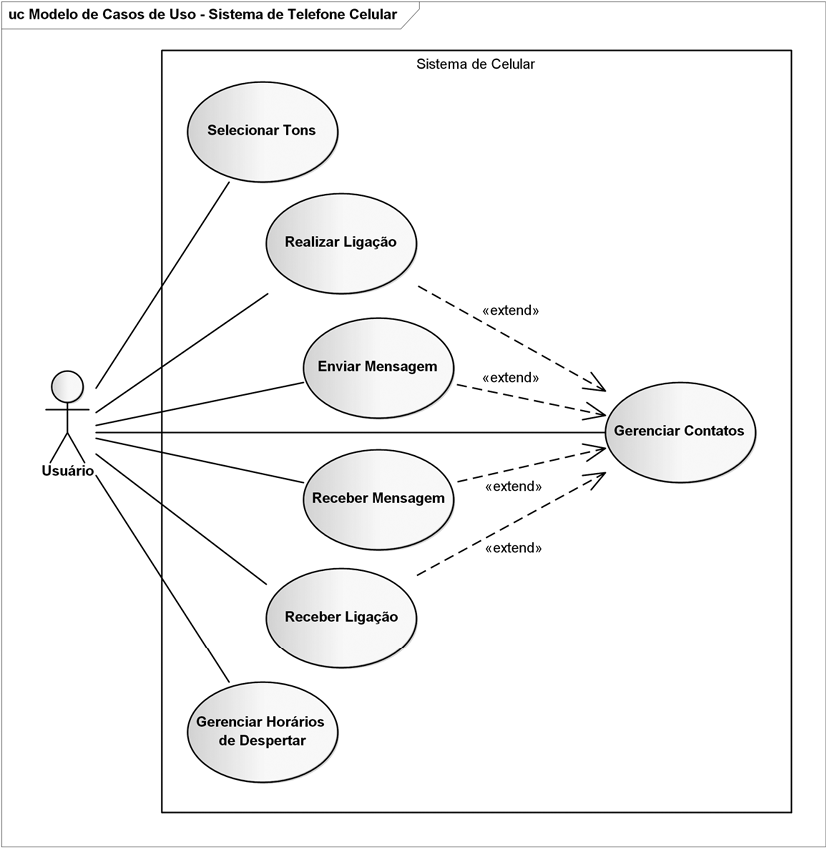
\includegraphics[width=0.92\textwidth,height=0.72\textheight,keepaspectratio]{imagens/Fig3.18.png}\\[0.1cm]
    \scriptsize Observe a divisão funcional entre serviços de voz, mensagens e utilitários e os múltiplos atores.
\end{frame}

% -----------------------------------------------------------------------------
% SLIDE 30: Estudo de Caso: Leilão Via Internet (Pagina Unica)
% -----------------------------------------------------------------------------
\begin{frame}{Estudo de Caso: Sistema de Leilão Via Internet}
    \centering
    \textbf{Diagrama para Sistema Web de Leilão (Figura 3.25 do Livro):}\\[0.15cm]
    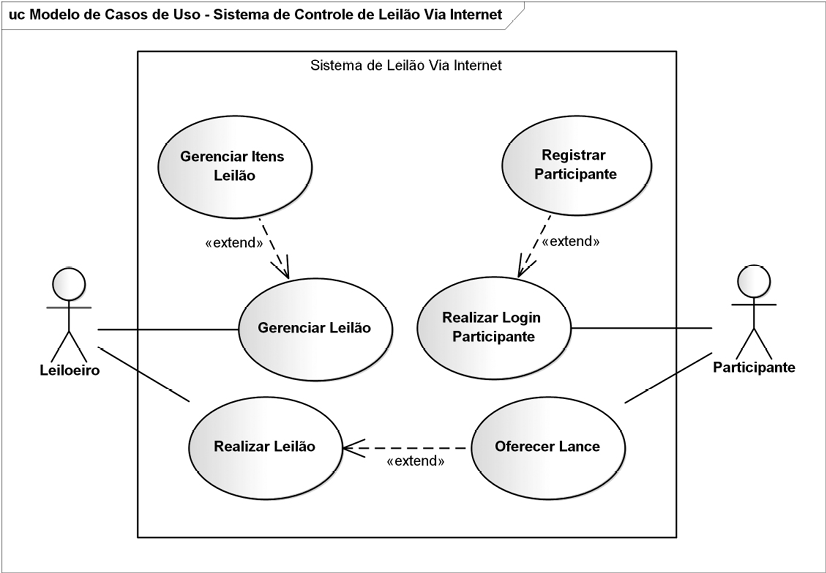
\includegraphics[width=0.92\textwidth,height=0.72\textheight,keepaspectratio]{imagens/Fig3.25.png}\\[0.1cm]
    \scriptsize Atores Comprador e Vendedor, Casos de Uso de lances, arremate, avaliação e notificações.
\end{frame}

% =============================================================================
\section{Atividade Prática e Exemplo de Modelagem}
% =============================================================================

% -----------------------------------------------------------------------------
% SLIDE 31: Atividade Pratica Proposta
% -----------------------------------------------------------------------------
\begin{frame}{Atividade Prática: Proposta e Requisitos}
    \begin{block}{Cenário: Sistema \textit{TauáDelivery Web}}
        Modelagem do Diagrama de Casos de Uso e documentação textual para delivery online.
    \end{block}
    \vspace{0.15cm}
    \begin{columns}
        \begin{column}{0.5\textwidth}
            \textbf{Requisitos a Modelar (RF01 a RF13):}
            \begin{itemize}
                \item \textbf{Atores:} Cliente, Entregador, Restaurante Parceiro e Gateway de Pagamento;
                \item \textbf{Casos de Uso:} Consultar Cardápio, Gerenciar Carrinho, Finalizar Pedido, Cancelar Pedido, Atualizar Status, etc.
                \item \textbf{Inclusões:} Finalizar Pedido inclui Autenticar e Processar Pagamento;
                \item \textbf{Extensões:} Finalizar Pedido estendido por Aplicar Cupom.
            \end{itemize}
        \end{column}
        \begin{column}{0.5\textwidth}
            \textbf{Entregáveis Solicitados:}
            \begin{enumerate}
                \item \textbf{Parte 1:} Análise conceitual de atores e relacionamentos;
                \item \textbf{Parte 2:} Diagrama de Casos de Uso completo com fronteira;
                \item \textbf{Parte 3:} Especificação técnica formal de \textit{UC03 - Finalizar Pedido} (Fluxos Principal, Alternativo e Exceção).
            \end{enumerate}
        \end{column}
    \end{columns}
\end{frame}

% -----------------------------------------------------------------------------
% SLIDE 32: Exemplo de Modelagem dos Requisitos RF01 e RF02 (Pagina Unica)
% -----------------------------------------------------------------------------
\begin{frame}{Exemplo de Modelagem: Requisitos RF01 e RF02}
    \centering
    \textbf{Diagrama de Casos de Uso para RF01 e RF02 (Modelo de Apoio):}\\[0.15cm]
    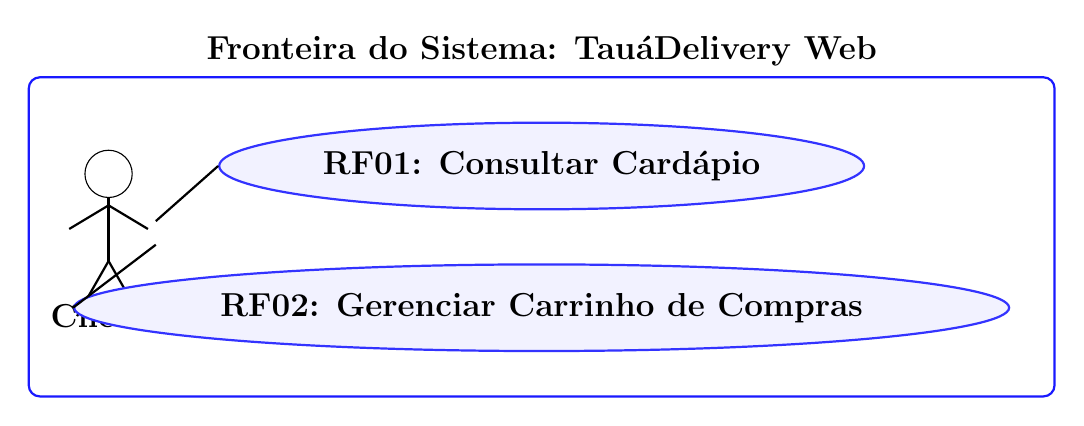
\includegraphics[width=0.92\textwidth,height=0.62\textheight,keepaspectratio]{imagens/modelagem_rf01_rf02.png}\\[0.15cm]
    \begin{block}{Comentário do Modelo de Referência}
        \scriptsize O ator \textbf{Cliente} conecta-se diretamente aos casos de uso \textbf{RF01: Consultar Cardápio} e \textbf{RF02: Gerenciar Carrinho de Compras}, ambos contidos dentro da \textbf{Fronteira do Sistema}.
    \end{block}
\end{frame}

% -----------------------------------------------------------------------------
% SLIDE 33: Especificação Textual de Apoio: UC01 e UC02
% -----------------------------------------------------------------------------
\begin{frame}{Especificação de Apoio: Casos de Uso UC01 e UC02}
    \begin{columns}
        \begin{column}{0.5\textwidth}
            \begin{block}{\scriptsize Ficha UC01 - Consultar Cardápio}
                \tiny
                \textbf{Ator:} Cliente \\
                \textbf{Pré-condição:} Sistema online com restaurantes cadastrados. \\
                \textbf{Pós-condição:} Cardápio exibido com fotos e preços. \\
                \textbf{Fluxo Principal:}
                1. Cliente acessa página inicial; \\
                2. Sistema lista restaurantes abertos; \\
                3. Cliente escolhe restaurante; \\
                4. Sistema exibe cardápio por categoria; \\
                5. Cliente clica no item para detalhes. \\
                \textbf{Fluxo Alternativo:} Busca por categoria ou prato. \\
                \textbf{Fluxo de Exceção:} Restaurante fora do horário de funcionamento.
            \end{block}
        \end{column}
        \begin{column}{0.5\textwidth}
            \begin{block}{\scriptsize Ficha UC02 - Gerenciar Carrinho}
                \tiny
                \textbf{Ator:} Cliente \\
                \textbf{Pré-condição:} Cliente visualizando cardápio (UC01). \\
                \textbf{Pós-condição:} Itens e valores totais calculados na sessão. \\
                \textbf{Fluxo Principal:}
                1. Cliente clica em ``Adicionar ao Carrinho''; \\
                2. Sistema valida disponibilidade e adiciona item; \\
                3. Sistema atualiza contador e subtotal; \\
                4. Cliente abre carrinho para conferência; \\
                5. Sistema lista itens, quantidades e total. \\
                \textbf{Fluxo Alternativo:} Alteração de quantidade ou remoção. \\
                \textbf{Fluxo de Exceção:} Alerta de troca de restaurante no carrinho.
            \end{block}
        \end{column}
    \end{columns}
    \vspace{0.2cm}
    \begin{alertblock}{Diretriz para os Alunos}
        Utilizem essa mesma estrutura formal para redigir o caso de uso \textbf{UC03: Finalizar Pedido}!
    \end{alertblock}
\end{frame}

% -----------------------------------------------------------------------------
% SLIDE 34: Conclusao e Proxima Aula
% -----------------------------------------------------------------------------
\begin{frame}{Conclusão e Próximos Passos}
    \begin{itemize}
        \item \textbf{A UML é a linguagem franca do software:} Permite pensar a arquitetura e alinhar requisitos antes de codificar.
        \item \textbf{A Orientação a Objetos é o alicerce:} Encapsulamento, herança e polimorfismo dão estrutura e flexibilidade ao domínio.
        \item \textbf{Casos de Uso definem o escopo do projeto:} Mapeiam de forma clara o que o software deve entregar do ponto de vista do usuário.
    \end{itemize}
    \vspace{0.3cm}
    \begin{exampleblock}{Próxima Aula (Aula 21)}
        \textbf{Aprofundamento no Diagrama de Classes e Diagrama de Atividades:}
        Associações complexas (multiplicidades, navegabilidade, agregação e composição) e modelagem de fluxos procedurais.
    \end{exampleblock}
\end{frame}

\end{document}
